\documentclass[10pt]{beamer}
\usetheme{metropolis}
\usepackage{appendixnumberbeamer}
\usepackage[utf8]{inputenc}
%\usepackage[T1]{fontenc}
\usepackage{lmodern}
\usepackage[french]{babel}
\usepackage{graphicx}

\usepackage{pgf,tikz}
\usetikzlibrary{calc,tikzmark}
\usetikzlibrary{quotes,angles}
\usetikzlibrary{arrows.meta,bending,automata,positioning}
\usetikzlibrary{shapes.geometric}
\usetikzlibrary{babel}
\usetikzlibrary{decorations.text}
\usetikzlibrary{matrix}
\usepackage{pgfplots}
\pgfplotsset{compat=1.14} 
%\usepackage[dvipsnames]{xcolor}
%\usepackage{textpos}
%\usepackage{tikz}
%\addtobeamertemplate{headline}{}{%
%\begin{textblock*}{100mm}(.85\textwidth,0cm)
%    \includegraphics[width=2cm]{fig/LOGO_ESME_QUADRI.EPS}
%\end{textblock*}}

%\addtobeamertemplate{block begin}{\setlength\abovedisplayskip{-1pt}}

%\definecolor{UBCblue}{rgb}{0.04706, 0.13725, 0.26667} % UBC Blue (primary)
%\usecolortheme[named=UBCblue]{structure}
%\setbeamertemplate{frametitle}{\color{black}\bfseries\insertframetitle\par\vskip-6pt\noindent\rule{0.8\textwidth}{.6pt}\hfil}

\title{Système automatiques}
\subtitle{Séance 1}
\date{}
\author{F. Vasconcelos}
\institute{ESME Sudria Lille}

\begin{document}
\maketitle

\metroset{background=dark}
\section{Un exemple historique \og classique\fg}
\metroset{background=light}

\begin{frame}
    \frametitle{Régulateur à boules de Watts}
    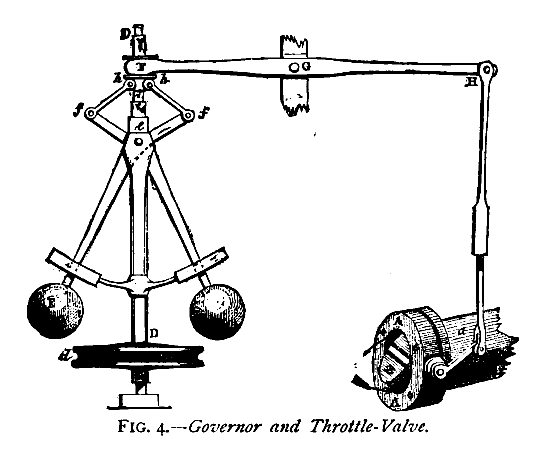
\includegraphics[width=\textwidth]{fig/Centrifugal_governor}
    \url{https://www.youtube.com/watch?v=SiYEtnlZLSs}
\end{frame}

\metroset{background=dark}
\section{Organisation du cours}
\metroset{background=light}

\begin{frame}
    \begin{figure}[!h]
        \begin{center}
            {
            \large
            \begin{tikzpicture}
\tikzset{box/.style={rectangle,
                     rounded corners=12pt,
                     minimum width=4.0cm,
                     minimum height=2cm}
}
\draw node[fill=col5!10!white,box] (A) at (0,0) {\scshape Automatique Linéaire};
\draw node[fill=col1!10!white,box] (M) at (-4.5,-2.8) {\scshape Modélisation}; 
\draw node[fill=col1!10!white,box] (N) at ( 0,-2.8) {\scshape Analyse}; 
\draw node[fill=col1!10!white,box] (S) at ( 4.5,-2.8) {\scshape Contrôle}; 
\draw[-latex,ultra thick] (A)--(M.north) ;
\draw[-latex,ultra thick] (A)--(N.north) ;
\draw[-latex,ultra thick] (A)--(S.north) ;
\tikzset{pos1/.style={fill=col1!10!white,
                      yshift=1.75em,
                      text width=4.0cm,
                      minimum height=4.5cm,
                      rounded corners=12pt}
}
\newcommand{\mysize}{\footnotesize}
\newcommand{\mysized}{\normalsize}
\node[below=of M,pos1] {\vbox {\mysize
                                    \begin{itemize}
                                        \item Mise en équation du système
                                        \item Modèles usuels
                                        \item Outils Mathématiques
                                    \end{itemize}}};
\node[below=of N,pos1] {\vbox {\mysize
                                    \begin{itemize}
                                        \item Réponses aux sollicitations
                                        \item Identification
                                        \item Caractérisation
                                        \item Performances
                                    \end{itemize}}};
\node[below=of S,pos1] {\vbox {\mysize
                                    \begin{itemize}
				        \item Consigne
				        \item Commande
					\item Asservissement
					\item Régulation
                                        \item Correction
                                    \end{itemize}}};
\tikzset{pos2/.style={fill=col4!10!white,
                      yshift=-10em,
                      text width=4.0cm,
                      minimum height=4cm,
                      rounded corners=12pt}
}
\node[below=of M,pos2] {\vbox {\mysized
                                    \begin{itemize}
                                        \item \Cref{chap-slci}
                                        \item \Cref{chap-schemabloc}
                                        \item \Cref{chap-model} 
                                        \item \Cref{chap-repreEtat} 
                                    \end{itemize}}};
\node[below=of N,pos2] {\vbox {\mysized
                                    \begin{itemize}
                                        \item \Cref{chap-repfreq}
                                        \item \Cref{chap-perf} 
                                        \item \Cref{chap-stab} 
                                    \end{itemize}}};
\node[below=of S,pos2] {\vbox {\mysized
                                    \begin{itemize}
                                        \item \Cref{chap-asservis} 
                                        \item \Cref{chap-correc} 
                                    \end{itemize}}};
\end{tikzpicture}

            }
        \end{center}
    \end{figure}  
\end{frame}

\begin{frame}
    \begin{figure}[!h]
        \begin{center}
            {
            \large
            \input{tikz/diagramme_cours_2.tex}
            }
        \end{center}
    \end{figure}  
\end{frame}


\end{document}
